\chapter{Noções sobre conjuntos no espaço euclidiano}

\resumo{titulo}{
\begin{itemize}[label=\color{chapterscolor}\textbullet]
  \item Compreensão dos conceitos fundamentais de conjuntos em $\mathbf{\R^n}$
  \item Identificação de diferentes tipos de conjuntos em $\R^2$ e $\R^3$
  \item Visualização geométrica de conjuntos em em $\R^2$ e $\R^3$
  \item Interpretação de notações envolvendo conjuntos em $\mathbf{\R^n}$
  \item Aplicação de conceitos de conjuntos em contextos práticos
  \item Identificação de conexões entre noções de conjuntos em $\R^n$ e outros tópicos matemáticos. 
\end{itemize}
}


Nesta primeira parte exploraremos os conjuntos no plano e no espaço, que são fundamentais para nosso curso de Cálculo II para economia. Compreender os conceitos básicos da topologia no espaço euclidiano é essencial para o estudo das funções de várias variáveis. 
%Aprenderemos coordenadas cartesianas, conjuntos de pontos e gráficos de funções, bem como operações e representações gráficas de conjuntos. Essas habilidades serão aplicadas na modelagem de situações econômicas e na otimização de recursos. Os conjuntos fornecerão uma base sólida para a análise rigorosa de fenômenos econômicos e a formulação de modelos precisos.

Começaremos lembrando que o símbolo \(\mathbb{R}^n\) representa o espaço euclidiano \(n\)-dimensional, também conhecido como espaço real \(n\)-dimensional, e é o conjunto das $n$-tuplas \(\Point{x}=(x_1, x_2, \ldots, x_n)\) em que cada coordenada \(x_i\) é um número real correspondente à coordenada do ponto no espaço. O índice \(n\) em \(\mathbb{R}^n\) indica o número de dimensões do espaço euclidiano. %Portanto, \(\mathbb{R}^n\) é um conjunto de vetores em um espaço \(n\)-dimensional, onde cada coordenada é um número real.



Por exemplo, \(\mathbb{R}^2\) representa o espaço euclidiano bidimensional, onde os pontos são representados por pares ordenados de números reais \((x, y)\) e podem ser visualizados como pontos em um plano cartesiano. Similarmente, \(\mathbb{R}^3\) representa o espaço tridimensional, onde os pontos são representados por triplas ordenadas de números reais \((x, y, z)\) e podem ser visualizados como pontos em um espaço tridimensional.
\begin{figure}[!htb]
    \centering
\begin{subfigure}{0.4\textwidth}
\centering
\begin{tikzpicture}[scale=0.6]
  \draw[-latex] (-4,0) -- (4,0) node[right]{$x$};
  \draw[-latex] (0,-4) -- (0,4) node[above]{$y$};
  
  \draw[gray!50,dashed] (2,3) -- (2,0) node[black,below]{$x$};
  \draw[gray!50,dashed] (2,3) -- (0,3) node[black,left]{$y$};

  \filldraw[red!150] (2,3) circle (1.5pt) node[above right]{$(x,y)$};
\end{tikzpicture}
\caption{O ponto $(2,3)$ em $\R^2$}
\end{subfigure}
\qquad\qquad
  \begin{subfigure}{0.4\textwidth}
    \centering
    \tdplotsetmaincoords{70}{110} % Define os ângulos de rotação
\begin{tikzpicture}[scale=0.7,tdplot_main_coords]
    % Eixos coordenados
    \draw[-latex] (0,0,0) -- (5,0,0) node[below] {$x$};
    \draw[-latex] (0,0,0) -- (0,5,0) node[right] {$y$};
    \draw[-latex] (0,0,0) -- (0,0,5) node[above] {$z$};
    
    % Ponto em R^3
    \coordinate (P) at (2,3,4);
    
    % Desenho do ponto
    \filldraw[red!150] (P) circle (2pt);
    
    % Rótulo do ponto
    \node[red!150,above right] at (P) {$(x,y,z)$};
    
    % Linhas guias
    \draw[gray!50,dashed] (0,0,4)--(P) -- (2,3,0)--(0,0,0);
    \draw[gray!50,dashed] (2,0,0) --(2,3,0)--(0,3,0);
    \draw (2,0,0) node[left]{$x$};
    \draw (0,3,0) node[above]{$y$};
    \draw (0,0,4) node[left]{$z$};
\end{tikzpicture}
\caption{O ponto $(2,3,4)$ em $\R^3$}
\end{subfigure}
\caption{Pontos no espaço euclidiano bi e tri-dimensional}
\label{fig:ex_pontos}
\end{figure}

Lembramos também que a distância entre dois pontos \(\Point{x}=(x_1, x_2, \ldots, x_n)\) e \(\Point{y}=(y_1, y_2, \ldots, y_n)\) no espaço euclidiano \(\mathbb{R}^n\) pode ser calculada utilizando a fórmula da distância entre dois pontos, dada por 
\[d(\Point{x},\Point{y}) = \sqrt{(x_1 - y_1)^2 + (x_2 - y_2)^2 + \ldots + (x_n - y_n)^2}.\] 
Claramente, a distância é sempre um valor não negativo e representa o comprimento do segmento de reta que conecta os dois pontos. Tal fórmula é uma generalização do Teorema de Pitágoras como pode ser observado na Figura \ref{exem:distancia}. 
\begin{figure}[!htb]
    \centering
    \tdplotsetmaincoords{70}{110} % Define os ângulos de rotação
\begin{tikzpicture}[scale=0.7,tdplot_main_coords]
    % Eixos coordenados
    \draw[-latex] (0,0,0) -- (5,0,0) node[below] {$x$};
    \draw[-latex] (0,0,0) -- (0,5,0) node[right] {$y$};
    \draw[-latex] (0,0,0) -- (0,0,5) node[above] {$z$};
    
    % Ponto em R^3
    \coordinate (P) at (2,3,4);
    \coordinate (O) at (0,0,0);
    
    % Desenho dos pontos
    \filldraw[red!150] (P) circle (2pt);
    \filldraw[red!150] (O) circle (2pt);
    
    % Rótulo dos pontos
    \node[red!150,right] at (P) {$p=(x,y,z)$};
    \node[red!150,left] at (O) {$O$};

    
    % Linhas guias
    \draw[gray!50,dashed] (0,0,4)--(P)node[midway,above,rotate=-25]{\footnotesize$\sqrt{x^2+y^2}$} -- (2,3,0)node[midway,right]{\footnotesize$z$}--(O);
    \draw[gray!50,dashed] (2,0,0) --(2,3,0)--(0,3,0);
%    \draw (2,0,0) node[left]{$2$};
%    \draw (0,3,0) node[above]{$2$};
%    \draw (0,0,4) node[left]{$2$};

% segmento que junta os pontos
\draw[red!150] (O)--(P); 
    
\end{tikzpicture}
\caption{$d(p,O)=\sqrt{x^2+y^2+z^2}$.}
\label{exem:distancia}
\end{figure}


\section{Conjuntos no espaço euclidiano}


\begin{definition}{Conjunto no espaço euclidiano}{def:conjunto}
Um \textit{conjunto no espaço euclidiano}\index{conjunto!no espaço euclidiano} \(\mathbb{R}^n\), é uma coleção de pontos em \(\mathbb{R}^n\). 
\end{definition}
Exemplos de conjuntos no plano são as retas e os círculos. As retas são os conjuntos de pontos cuja ordenada $y$ satisfaz uma equação do tipo
\begin{equation}\label{eq:reta}
    y=m\,x+b,
\end{equation}
onde $m$ e $b$ são constantes que representam, respectivamente, a inclinação da reta com respeito ao eixo $x$ é o ponto onde a reta intercepta o eixo $y$ (também conhecido como intercepto $y$). Ou seja, a reta $r$ de equação \eqref{eq:reta} é o conjunto
\[r=\left\{(x,y)\in \R^2; y=m\,x+b\right\}\equiv \left\{(x,m\,x+b)\in \R^2\right\}.\]

\pagebreak

Os círculos, por sua vez, são conjuntos do plano que consistem em todos os pontos que estão a uma distância fixa de um certo ponto, chamado centro do círculo. Essa distância é chamada de raio do círculo. Matematicamente, um círculo $C$ com centro em $(h,k)$ e raio $r$ pode ser descrito pela equação
\begin{equation}\label{eq:circulo}
    (x - h)^2 + (y - k)^2 = r^2.
\end{equation}
Essa equação representa todos os pontos $(x,y)$ no plano cartesiano cuja distância até o ponto $(h,k)$ é \textit{igual} ao raio $r$. Ou seja, 
$$C=\left\{(x,y)\in\R^2; (x - h)^2 + (y - k)^2 = r^2 \right\}.$$
Na Figura \ref{fig:2} mostramos dois exemplos de conjuntos no plano.  
O primeiro é a reta $r$ que une os pontos $(0,0)$ e $(2,3)$ (Figura \ref{fig:2-reta_r}), ou seja, o conjunto
\[r=\left\{(x,y)\in \R^2; y=3/2\,x\right\}\equiv \left\{(x,3/2\,x)\in \R^2\right\}.\]
O segundo é o círculo 
$$C=\left\{(x,y)\in\R^2;~x^2+y^2=1\right\},$$
isto é, o conjunto de pontos no plano que está a uma distância da origem de 1 unidade (Figura \ref{fig:2-circulo}). 
\begin{figure}[!htb]
  \centering
  \begin{subfigure}{0.4\textwidth}
    \centering
\begin{tikzpicture}
  \draw[-latex] (0,0) -- (4,0) node[right]{$x$};
  \draw[-latex] (0,0) -- (0,4) node[above]{$y$};
  
  \draw[dashed] (2,3) -- (2,0) node[below]{2};
  \draw[dashed] (2,3) -- (0,3) node[left]{3};

\draw[green!150,shorten >= -1.5cm,shorten <= -0.5cm] (0,0)-- (2,3) node[midway,above]{$r$};


  \filldraw[red!150] (2,3) circle (1.5pt) node[right]{$(2,3)$};
  \filldraw[red!150] (0,0) circle (1.5pt) node[left]{$(0,0)$};

\end{tikzpicture}
    \caption{A reta $r$}
    \label{fig:2-reta_r}
  \end{subfigure}
  \hfill
\begin{subfigure}{0.4\textwidth}
    \centering
\begin{tikzpicture}[scale=1.1]
  \draw[-latex] (-2,0) -- (2,0) node[right]{$x$};
  \draw[-latex] (0,-2) -- (0,2) node[above]{$y$};
\draw[green!150] (0,0) circle [radius=1];
\draw[green!150] (45:.9) node[above right]{$C$};

%\draw (0,0) circle (1.5pt) node{};
\draw (1,0) node[below right]{\footnotesize $1$};
\draw (-1,0) node[below left]{\footnotesize $-1$};
\draw (0,1) node[above left]{\footnotesize $1$};
\draw (0,-1) node[below left]{\footnotesize $-1$};

\end{tikzpicture}
    \caption{O cículo $C$}
    \label{fig:2-circulo}
  \end{subfigure}
  \caption{Exemplos de conjuntos no plano}
  \label{fig:2}
\end{figure}


Como vimos, as retas e os círculos são descritas por uma determinada relação ou equação. %Vale ressaltar que nem toda curvas no plano pode ser descrita por uma única relação entre as variáveis $x$ e $y$, como é o caso de algumas  \textit{curvas transcendentes}, tais como a \textit{cicloide} e a \textit{Lemniscata de Bernoulli} representadas na Figura \ref{fig:curvas_trascendentes}. Algumas dessas curvas serão estudadas no tópico de  \textit{Curvas parametrizadas}. 
Observe, porém, que ao contrário do que ocorre com as retas (vide equação \eqref{eq:reta}), no podemos expressar na relação \eqref{eq:circulo} a variável $y$ em função de $x$ em apenas uma equação, e vice-versa, porque tal relação contém termos quadráticos em ambas as variáveis. De fato, se quisermos expressar $y$ em função de $x$, por exemplo, obtém-se
\[y=\pm \sqrt{r^2-(x-h)^2}+k.\]

Lembramos que uma equação com essas características é chamada de \textit{equação implícita}\index{equação!implícita}. Em geral, uma \textit{equação implícita}\index{equação!implícita} em $n$ variáveis é uma equação em que não é possível expressar nenhuma das variáveis envolvidas na equação \textit{explicitamente} em função das outras. %No caso contrário dizemos que a equação é uma \textit{equação explícita}\index{equação!explícita}. 
%Conjuntos no plano dados por equações são exemplos de curvas. 



No espaço euclidiano tridimensional também conhecemos vários exemplos de conjuntos cujos pontos satisfazem uma determinada relação entre suas coordenadas. Por exemplo, os planos são descritos por uma equação linear da forma
\begin{equation}\label{eq:plano}
    a\,x+b\;y +c\, z =d,
\end{equation}
onde $a$, $b$, $c$ e $d$ são constantes reais. %Ou seja, os planos são conjuntos em $\R^3$ da forma
%$$\{(x,y,z)\in\R^3;~ ax+by+cz=d\}.$$
Na Figura \ref{exem:plano} está representado o plano cuja equação é $x+y+z=2$, ou seja, o conjunto de pontos
$$P=\left\{(x,y,z)\in\R^3;~x+y+z=2\right\}.$$
%\vspace*{-1cm}
\begin{figure}[!htb]
\centering
\tdplotsetmaincoords{70}{110} % Define a perspectiva do plano 3D
\begin{tikzpicture}[scale=1.25,tdplot_main_coords]
    % Eixos coordenados
    \draw[-latex] (0,0,0) -- (3,0,0) node[below] {$x$};
    \draw[-latex] (0,0,0) -- (0,3,0) node[right] {$y$};
    \draw[-latex] (0,0,0) -- (0,0,3) node[above] {$z$};
    
    % Pontos que definem o plano
    \coordinate (A) at (0,0,2);
    \coordinate (B) at (2,0,0);
    \coordinate (C) at (0,2,0);
    
    % Desenho do plano
    \draw[blue,dashed,fill=blue!10,opacity=0.75] (A) -- (B) -- (C) -- cycle;
    
    
    
    % Rótulos dos pontos
    \node[left] at (A) {\footnotesize$2$};
    \node[left] at (B) {\footnotesize$2$};
    \node[above right] at (C) {\footnotesize$2$};
\end{tikzpicture}
\caption{Representação no primeiro quadrante do plano cuja equação é $x+y+z=2$.}
\label{exem:plano}
\end{figure}

Outro exemplo é a esfera, que, analogamente ao círculo no plano, é o conjunto dos pontos que equidistam de um ponto fixo chamado centro: 
\begin{equation}\label{eq:esfera}
    \left\{(x,y,z)\in\R^3;~ (x-x_0)^2+(y-y_0)^2+(z-z_0)^2=r^2\right\},
\end{equation}

Na Figura \ref{fig:esfera} temos a esfera centrada na origem e de raio $1$, ou seja, o conjunto de pontos em $\R^3$ que está a uma distância fixa de 1 unidade da origem.  
%\todo[inline]{Mais exemplos de conjuntos que são superfícies no espaço}
\begin{figure}[!htb]
    \centering
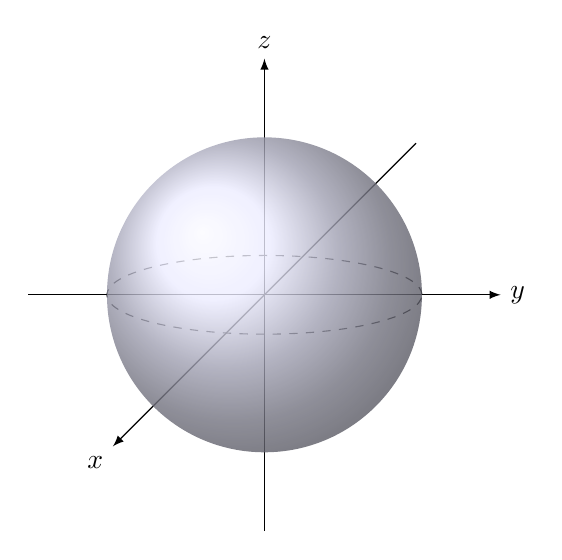
\begin{tikzpicture}
  \begin{scope}[scale=1,cm={-1,-1,1,0,(0,0)},x=3.85mm,z=-1cm]
    \draw[-latex] (-5,0,0) -- (5,0,0) node[anchor=north east]{$x$};
    \draw[-latex] (0,-3,0) -- (0,3,0) node[right]{$y$};
    \draw[-latex] (0,0,-3) -- (0,0,3) node[above]{$z$};
  \end{scope}
\draw[dashed] (0,0) ellipse (2 and .5);
\shade[ball color=blue!100!blue!10!white,opacity=.8] (0,0,0) circle (2);
\end{tikzpicture}
\caption{A esfera de equação $x^2+y^2+z^2=1$.}
    \label{fig:esfera}
\end{figure}


Os planos e as esferas são exemplos muito particulares do que chamamos de \textit{superfícies}\index{superfícies}.  
Neste curso não daremos uma definição rigorosa do conceito de  superfície, pois carecemos de ferramentas matemáticas para tal abordagem. Em vez disso, \textit{assumiremos que uma superfície é um conjunto de pontos em $\R^3$ que satisfazem uma determinada relação entre suas coordenadas}. Tal equação pode ser \textit{explícita} -- como no caso do plano -- ou \textit{implícita} --como no caso da esfera, dependendo da natureza da superfície. 

Até o momento, estudamos conjuntos no plano e no espaço que podem ser descritos por uma única equação relacionando suas coordenadas. Esses conjuntos são de extrema importância neste curso, pois se tratam dos chamados \textit{conjuntos de nível} de funções de duas e três variáveis. Esses conjuntos desempenham um papel fundamental na resolução de problemas de otimização com restrições.


%Nos exemplos acima citados vemos que os planos são superfícies dadas por equações explícitas, já que, por exemplo, a altura $z$ pode ser escrita explicitamente em termos de $x$ e $y$. Pelo contrário, a esfera é uma superfície dada por uma equação implícita, pois nenhuma das variáveis pode ser expressa explicitamente em função das outras duas. 



%No entanto, nem toda superfície em $\R^3$ pode ser descrita por uma equação, nem que seja implícita, como é o caso da \textit{Garrafa de Klein}, mas, obviamente, tais superfícies fogem do objetivo do nosso curso. 
%\todo[inline]{Garrafa de Klein}
\begin{comment}
    \begin{figure}[!htb]
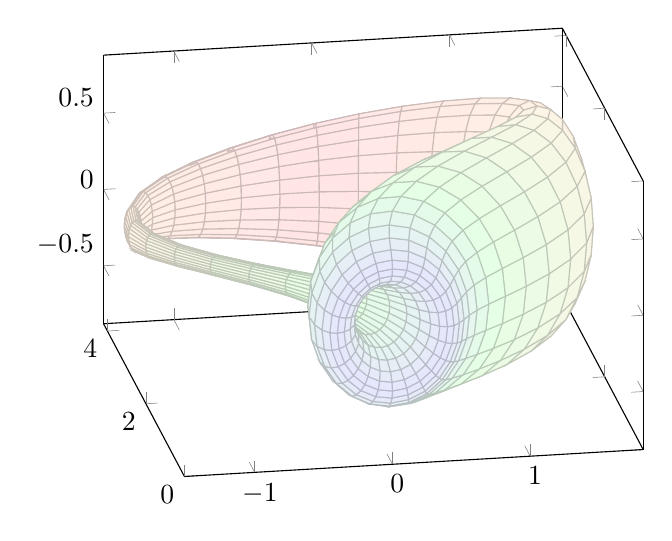
\begin{tikzpicture}
	\begin{axis}[
%            view={130}{30},
%            axis lines=none,
%		xlabel=$x$,
%		ylabel=$y$,
		view/h=-10,
%		title=\footnotesize 
 %\url{http://en.wikipedia.org/wiki/Klein_bottle},
	]
	\addplot3[
		surf,
		z buffer=sort,
		colormap={periodic}{%
			color=(blue!10) 
			   color=(green!10) 
			      color=(orange!10) 
				     color=(red!10)
			      color=(orange!10) 
	           color=(green!10) 
	        color=(blue!10)},
		domain=0:180, domain y=0:360,
		samples=41, samples y=25,
		variable=\u, variable y=\v,
		point meta=u,
		] 
		({-2/15 * cos(u) * (
		    3*cos(v) - 30*sin(u) 
		  + 90 *cos(u)^4 * sin(u) 
		  - 60 *cos(u)^6 * sin(u)  
		  + 5 * cos(u)*cos(v) * sin(u))
		 },
		 {-1/15 * sin(u) * (3*cos(v) 
		  - 3*cos(u)^2 * cos(v) 
		  - 48 * cos(u)^4*cos(v) 
		  + 48*cos(u)^6 *cos(v) 
		  - 60 *sin(u) 
		  + 5*cos(u)*cos(v)*sin(u) 
		  - 5*cos(u)^3 * cos(v) *sin(u) 
		  - 80*cos(u)^5 * cos(v)*sin(u) 
		  + 80*cos(u)^7 * cos(v) * sin(u))
		 },
		 {2/15 * (3 + 5*cos(u) *sin(u))*sin(v)});
	\end{axis}
\end{tikzpicture}
\caption[Garrafa de Klein]{Garrafa de Klein\footnotemark}
\label{fig:Klein}
\end{figure}
\footnotetext{Adaptado de \url{https://pgfplots.net/klein-bottle/}}
\end{comment}

\subsection{Regiões no plano e no espaço}
%Até aqui vimos vários exemplos de conjuntos que foram estudados no primeiro período na disciplina de \textit{Geometria Analítica}. 

%Além dos conjuntos estudados até aqui, podemos encontrar outros conjuntos com geometrias mais complexas. 

A modo de motivação, queremos saber como poderíamos representar \textit{analiticamente} o conjunto dos pontos que estão dentro do círculo $C$ da Figura \ref{fig:2-circulo}? Para isto, basta observar que qualquer ponto $p=(x,y)$ nesse conjunto está sobre um círculo centrado na origem cujo raio $r$ é estritamente menor do que $1$ (vide Figura \ref{fig:2-circulo_2}), isto é, $x^2+y^2=r^2<1$. 
Tal conjunto é a \textit{bola de raio 1 centrada na origem}\index{bola} e será denotado por $B(O,1)$, onde $O$ denota a origem:
$$B(O,1) =\left\{(x,y)\in\R^2;~x^2+y^2<1\right\},$$
\begin{figure}[!htb]
    \centering
\begin{tikzpicture}[scale=1.25]

  \draw[-latex] (-2,0) -- (2,0) node[right]{$x$};
  \draw[-latex] (0,-2) -- (0,2) node[above]{$y$};

\draw[green!150,dashed,fill=green!10,opacity=0.75] (0,0) circle [radius=1];
%\draw[green!150] (45:.9) node[above right]{$C$};

\draw[red!150] (0,0) circle [radius=.5];
\draw[red!150] (45:.4) node[above right]{\small $(x,y)$};
\filldraw[red!150] (45:.5) circle (1.5pt);


%\draw (0,0) circle (1.5pt) node{};
\draw (1,0) node[below right]{\footnotesize $1$};
\draw (-1,0) node[below left]{\footnotesize $-1$};
\draw (0,1) node[above left]{\footnotesize $1$};
\draw (0,-1) node[below left]{\footnotesize $-1$};

\end{tikzpicture}
    \caption{A bola $B(O,1)$ de raio 1 e o ponto $(x,y)$ dentro do círculo.}
    \label{fig:2-circulo_2}
  \end{figure}


O conjunto $B(O,1)$ acima é um exemplo de uma bola aberta. De forma geral, uma \textit{bola aberta}\index{bola!aberta} é uma região geométrica no espaço euclidiano \(\mathbb{R}^n\) que consiste em todos os pontos que estão a uma distância menor que um determinado raio positivo de um ponto central especificado. Mais precisamente, dado um ponto $\Point{x}=(x_1,x_2,\dots,x_n)\in\R^n$, a bola aberta de raio $\varepsilon>0$ centrada em $x$ é denotada por \(B(x, \varepsilon)\) e é definida como:
\[B(x, \varepsilon) = \{y=(y_1,y_2,\dots,y_n) \in \mathbb{R}^n ;~ \text{dist}(x, y) < \varepsilon\},\]
onde \(\text{dist}(x, y)\) representa a distância entre os pontos \(x\) e \(y\) em \(\mathbb{R}^n\).


Por exemplo, o conjunto dos pontos que estão dentro da esfera 
da Figura \ref{fig:esfera} é a bola aberta 
\[B(O, 1) = \{(x,y,z)\in\R^3 ;~x^2+y^2+z^2 < 1\},\]
onde $O$ é a origem do espaço euclidiano tridimensional. 


Tendo o conceito de bola aberta podemos definir um conjunto aberto de forma geral. 

\begin{definition}{Conjunto aberto}{def:conjunto_aberto}
Um conjunto \(D\) no espaço euclidiano \(\mathbb{R}^n\) é chamado de \textit{conjunto aberto}\index{conjunto!aberto} se, %para cada ponto \(x\) em \(D\), existe um raio positivo \(\varepsilon > 0\) tal que todos os pontos do espaço euclidiano que estão a uma distância menor que \(\varepsilon\) de \(x\) também pertencem a \(D\).     
para cada ponto \(x\) em \(D\), existe uma bola aberta centrada em \(x\) totalmente contida em \(D\).
\end{definition}

\begin{exercise}{}{exer:bolas_abertas}
Mostre que as bolas abertas são conjuntos abertos. 

\dica 
Considere um ponto qualquer na bola, por exemplo, \((x_0, y_0)\), e faça a escolha de um raio \(r_0 > 0\) tal que a bola aberta \(B((x_0, y_0), r_0)\) esteja completamente contida nela. 
\end{exercise}



E o que acontece se ``juntarmos'' o círculo $C$ à bola aberta $B(O,1)$? Ou seja, se considerarmos o conjunto 
\[\overline{B(O, 1)} = \{(x,y,z)\in\R^3 ;~x^2+y^2 \leq 1\}.\]
Esse conjunto já não seria um conjunto aberto. Pois qualquer bola centrada em pontos de $C$ contêm pontos que não estão em $\overline{B(O,1)}$, como mostra a Figura \ref{fig:disco_fechado}. 
\begin{figure}[!htb]
\centering
\begin{tikzpicture}[scale=1.1]

\draw[green!150,fill=green!10] (0,0) circle [radius=1];
%\draw[green!150] (45:.9) node[above right]{$C$};


  \draw[-latex] (-2,0) -- (2,0) node[right]{$x$};
  \draw[-latex] (0,-2) -- (0,2) node[above]{$y$};


\draw[dashed, red!150, fill=red!20,opacity=0.5] (45:1) circle [radius=.35];
\draw[red!150] (45:1.1) node[below left]{\small $p$};
\draw[red!150] (45:1.35) node[right]{\small $B(p,\varepsilon)$};

\filldraw[red!150] (45:1) circle (1.5pt);


%\draw (0,0) circle (1.5pt) node{};
\draw (1,0) node[below right]{\footnotesize $1$};
\draw (-1,0) node[below left]{\footnotesize $-1$};
\draw (0,1) node[above left]{\footnotesize $1$};
\draw (0,-1) node[below left]{\footnotesize $-1$};

\end{tikzpicture}
\caption{}
  \label{fig:disco_fechado}
\end{figure}


\pagebreak
Esse conjunto, na verdade, é um conjunto fechado. Mas para definirmos formalmente o que é um \textit{conjunto fechado}, precisamos introduzir primeiro o conceito de complemento de um conjunto. 
\begin{definition}{Complemento de um conjunto}{def:complemento}
O \textit{complemento de um conjunto}\index{complemento de um conjunto}\index{conjunto!complemento de um} \(D\in\R^n\), denotado por \(D^c\), é o conjunto de todos os pontos que não pertencem a \(D\).
%, isto é, 
%\[D^c = \left\{x \in \mathbb{R}^n ;~ x \notin D\right\}.\]
\end{definition}


Por exemplo, o complementar da bola aberta $B(O,1)$ representada na Figura \ref{fig:2-circulo_2} é o conjunto de pontos 
$$ B(O,1)^c= \left\{(x,y)\in\R^2;~x^2+y^2 \geq 1\right\}.$$
De fato, seguindo o mesmo raciocínio que antes, qualquer ponto $(x,y)\in B(O,1)^c$ está em uma circunferência de raio $r\geq 1$ como se mostra na Figura \ref{fig:2-circulo_3} (lembre que a circunferência de raio 1 não faz parte da bola aberta $B(O,1)$.) 
\begin{figure}[!htb]
    \centering
\begin{tikzpicture}[scale=1.25]

\draw[blue!10, fill=blue!10] (-2,-2) rectangle (2,2);
\draw[thick,blue!140,fill=white] (0,0) circle [radius=1];

  \draw[-latex] (-2,0) -- (2,0) node[right]{$x$};
  \draw[-latex] (0,-2) -- (0,2) node[above]{$y$};



%\draw[green!150] (45:.9) node[above right]{$C$};

\draw[red!150] (0,0) circle [radius=1.5];
\draw[red!150] (45:1.5) node[above right]{\small $(x,y)$};
\filldraw[red!150] (45:1.5) circle (1.5pt);


%\draw (0,0) circle (1.5pt) node{};
\draw (1,0) node[below right]{\footnotesize $1$};
\draw (-1,0) node[below left]{\footnotesize $-1$};
\draw (0,1) node[above left]{\footnotesize $1$};
\draw (0,-1) node[below left]{\footnotesize $-1$};
\end{tikzpicture}
    \caption{Representação de $B(O,1)^c$ e um ponto $(x,y)\in B(O,1)^c$.}
    \label{fig:2-circulo_3}
  \end{figure}
%\footnotetext{Observe que na figura o círculo $C$ está tracejado queremos representar apenas os pontos que estão dentro do círculo.}  

\begin{definition}{Conjunto fechado}{def:conj_fechado}
Dizemos que um conjunto $D\in\R^n$ é um \textit{conjunto fechado}\index{conjunto!fechado} se $D^c$ é um conjunto aberto.     
\end{definition}

\newpage 
Assim, $B(O,1)^c$ é fechado pois o complemento de $B(O,1)^c$ é $B(O,1)$, que é um conjunto aberto. Também é fechado o conjunto $\overline{B(O,1)}$, pois seu complementar é o conjunto
$$ \overline{B(O,1)}^c= \left\{(x,y)\in\R^2;~x^2+y^2 > 1\right\}.$$


Por outro lado, temos observado como o círculo $C$ representa ``uma fronteira'' entre $B(O,1)$ e $B(O,1)^c$. Intuitivamente, vemos que toda bola centrada em qualquer ponto $p\in C$ contêm pontos que estão em $B(O,1)$ e em $B(O,1)^c$ (Vide Figura \ref{fig:2-circulo_4}). De modo geral podemos definir o conceito de fronteira. 
\begin{definition}{Fronteira de um conjunto}{def:fronteira}
\begin{comment}
A \textit{fronteira de um conjunto}\index{fronteira de um conjunto}\index{conjunto!fronteira de um} \(D\in\R^n\) é definida por:
\[\partial D = \{x \in \mathbb{R}^n ;~ \forall \varepsilon > 0~ B(x, \varepsilon) \cap D \neq \emptyset \text{ e } B(x, \varepsilon) \cap (D^c) \neq \emptyset\},\]
onde \(B(x, \varepsilon)\) é a bola aberta centrada em \(x\) com raio \(\varepsilon\) e \(\emptyset\) representa o conjunto vazio.
\end{comment}
A \textit{fronteira de um conjunto}\index{fronteira de um conjunto}\index{conjunto!fronteira de um} \(D\in\R^n\) é o conjunto dos pontos tais que \textit{toda} bola aberta que tem o ponto como centro contêm pontos que estão tanto em $D$ quanto em $D^c$.
\end{definition}

\begin{figure}[!htb]
    \centering
\begin{tikzpicture}[scale=1.25]

\draw[blue!10, fill=blue!10] (-2,-2) rectangle (2,2);
\draw[blue!140] (45:2) node{\footnotesize $B(O,1)^c$};

\draw[thick,blue!140,fill=green!10] (0,0) circle [radius=1];
\draw[green!150] (30:0.5) node{\footnotesize $B(O,1)$};


\draw[-latex] (-2,0) -- (2,0) node[right]{$x$};
\draw[-latex] (0,-2) -- (0,2) node[above]{$y$};



\draw[blue!140] (45:.9) node[above right]{$C$};


\draw[dashed,red!150] (90+45:1) circle [radius=.35];

\filldraw[red!150] (90+45:1) circle (1pt) node[below]{\footnotesize $p$};


%\draw[red!150] (0,0) circle [radius=1.5];
%\draw[red!150] (45:1.5) node[above right]{\small $(x,y)$};
%\filldraw[red!150] (45:1.5) circle (1.5pt);



%\draw (0,0) circle (1.5pt) node{};
\draw (1,0) node[below right]{\footnotesize $1$};
\draw (-1,0) node[below left]{\footnotesize $-1$};
\draw (0,1) node[above left]{\footnotesize $1$};
\draw (0,-1) node[below left]{\footnotesize $-1$};
\end{tikzpicture}
%\caption{}
\caption[O círculo como fronteira de $B(O,1)$]{O círculo como fronteira de $B(O,1)$\footnotemark.}
    \label{fig:2-circulo_4}
  \end{figure}
\footnotetext{Observe que $C$ também é a fronteira de $B(O,1)^c$.}  


\begin{comment}
\begin{definition}{Fecho de um conjunto}{def:fecho_conjunto}
O \textit{fecho de um conjunto}\index{fecho de um conjunto}\index{conjunto!fecho de um} é o conjunto 
    $$\overline{D} = D \cup \partial D.$$
\end{definition}
Não será mostrado aqui mas, de fato, $\overline{D}$ é um conjunto fechado. De maneira muito simplificada, como vimos no caso da bola aberta $B(O,1)$, sempre que ``juntemos'' um conjunto a sua fronteira, o resultado é um conjunto fechado. 
\end{comment}

\newpage 
\begin{exercise}{}{}
    \begin{enumerate}[label=\color{green!140}(\alph*)]
\item Mostre que um conjunto é fechado se ele contêm \textit{todos} os seus pontos de fronteira.
\item Mostre que um conjunto é aberto se ele não contêm \textit{nenhum} ponto de fronteira. 
\item Ilustre com um exemplo no plano ou no espaço que os conceitos de \textit{aberto} e \textit{fechado} não são excludentes, ou seja, que se um conjunto não é aberto não necessariamente será fechado, e vice-versa. 
\end{enumerate}
\end{exercise}

Por outro lado, o interior de um conjunto pode ser compreendido como o conjunto de pontos que estão ``bem dentro'' do conjunto, ``afastados'' de sua fronteira. 
\begin{definition}{Interior de um conjunto}{def:interior_conjunto}
O  \textit{interior}\index{interior de um conjunto}\index{conjunto!interior de um} de um conjunto \(D\in\R^n\), denotado por \(D^\circ\), é o conjunto de todos os pontos em \(D\) para os quais é possível encontrar uma bola aberta com centro no ponto e raio positivo completamente contida em \(D\). 
\begin{comment}
Isto é,
\[D^\circ = \{\Point{x}=(x_1,x_2,\dots, x_n) \in D \,;\, \exists r > 0 \text{ tal que } B(x, r) \subset A\}\]
\end{comment}
\end{definition}

\newpage 
Intuitivamente, se um ponto do conjunto está afastado\footnote{No contexto matemático, estar \textit{afastado} ou \textit{longe} de alguma referência significa estar a uma distância positiva dela, mesmo que tal distância seja pequena.} da sua fronteira, então tem vizinhos muito próximos que também estão afastados da fronteira (Figura \ref{fig:2-circulo_5}). 

\begin{figure}[!htb]
    \centering
\begin{tikzpicture}[scale=2]

\draw[dashed,green!150,fill=green!10] (0,0) circle [radius=1];
%\draw[green!150] (30:1.5) node{\footnotesize $B(O,1)$};


\draw[-latex] (-1.5,0) -- (1.5,0) node[right]{$x$};
\draw[-latex] (0,-1.5) -- (0,1.5) node[above]{$y$};



\draw[dash pattern= on 2pt off 2pt,red!75] (90+45:.85) circle [radius=.10] ;
\filldraw[red!140] (90+45:.85) circle (.25pt);

\draw[dash pattern= on 2pt off 2pt,blue!140] (45:.65) circle [radius=.25] ;
\filldraw[blue!140] (45:.65) circle (.45pt);


\draw[dash pattern= on 2pt off 2pt,orange] (-135:.20) circle [radius=.7] ;
\filldraw[orange] (-135:.20) circle (.45pt);



%\draw[red!150] (0,0) circle [radius=1.5];
%\draw[red!150] (45:1.5) node[above right]{\small $(x,y)$};
%\filldraw[red!150] (45:1.5) circle (1.5pt);



%\draw (0,0) circle (1.5pt) node{};
\draw (1,0) node[below right]{\footnotesize $1$};
\draw (-1,0) node[below left]{\footnotesize $-1$};
\draw (0,1) node[above left]{\footnotesize $1$};
\draw (0,-1) node[below left]{\footnotesize $-1$};
\end{tikzpicture}
\caption{$B(O,1)^\circ=B(O,1)$.}
    \label{fig:2-circulo_5}
  \end{figure}





Porém, existem conjuntos nos quais não ``cabe'' nenhuma bola, como é o caso das retas e dos círculo -- e das curvas em geral (vide Figura \ref{fig:2_fechado}). Neste caso dizemos que o interior do conjunto é vazio. Deixamos aos leitores verificarem que os planos e as esferas são conjuntos com interior vazio em $\R^3$, assim como todas as superfícies. 
%Por outro lado, os conjuntos representados na Figura \ref{fig:2} não são conjuntos abertos, pois, em ambos os casos, para qualquer ponto $p$ no conjunto e qualquer raio positivo $\varepsilon>0$, a bola aberta $B(p,\varepsilon)$ contem pontos que não pertencem ao conjunto (vide Figura \ref{fig:2_fechado}). \ref{fig:2-circulo_5}. 
\begin{figure}[!htb]
  \centering
  \begin{subfigure}{0.4\textwidth}
    \centering
\begin{tikzpicture}
  \draw[-latex] (0,0) -- (4,0) node[right]{$x$};
  \draw[-latex] (0,0) -- (0,4) node[above]{$y$};
  
%  \draw[dashed] (2,3) -- (2,0) node[below]{2};
%  \draw[dashed] (2,3) -- (0,3) node[left]{3};

\draw[green!150,shorten >= -1.5cm,shorten <= -0.5cm] (0,0)-- (2,3);


%  \filldraw[red!150] (2,3) circle (1.5pt) node[right]{$(2,3)$};
%  \filldraw[red!150] (0,0) circle (1.5pt) node[left]{$(0,0)$};

\draw[dashed, red!150, fill=red!20,opacity=0.5] (2,3) circle [radius=.5] ;
\draw[red!150] (2,3) node[below]{\small $p$};
\filldraw[red!150] (2,3) circle (1.5pt);
\draw[red!150] (3,3) node{\small $B(p,\varepsilon)$};
\end{tikzpicture}
    \caption{A reta $r$}
    \label{fig:2-reta_r_fechado}
  \end{subfigure}
  \hfill
\begin{subfigure}{0.4\textwidth}
    \centering
\begin{tikzpicture}[scale=1.1]

  \draw[-latex] (-2,0) -- (2,0) node[right]{$x$};
  \draw[-latex] (0,-2) -- (0,2) node[above]{$y$};

\draw[green!150] (0,0) circle [radius=1];
%\draw[green!150] (45:.9) node[above right]{$C$};

\draw[dashed, red!150, fill=red!20,opacity=0.5] (45:1) circle [radius=.35];
\draw[red!150] (45:1.1) node[below left]{\small $p$};
\draw[red!150] (45:1.35) node[right]{\small $B(p,\varepsilon)$};

\filldraw[red!150] (45:1) circle (1.5pt);


%\draw (0,0) circle (1.5pt) node{};
\draw (1,0) node[below right]{\footnotesize $1$};
\draw (-1,0) node[below left]{\footnotesize $-1$};
\draw (0,1) node[above left]{\footnotesize $1$};
\draw (0,-1) node[below left]{\footnotesize $-1$};

\end{tikzpicture}
    \caption{O cículo $C$}
    \label{fig:2-circulo_fechado}
  \end{subfigure}
  \caption{Conjuntos com interior vazio.}
  \label{fig:2_fechado}
\end{figure}

 


Continuando a extrair mais intuições da reta e do círculo, podemos perceber que a reta é um conjunto que se estende infinitamente em ambas as direções. Já o círculo está contido em uma região finita do plano. Enquanto a reta é um exemplo clássico de um \textit{conjunto ilimitado}, o círculo é um exemplo do que chamamos de \textit{conjunto limitado}.
\begin{definition}{Conjunto limitado}{def:conj_limitado}
Dizemos que $D\in\R^n$ é um \textit{conjunto limitado}\index{conjunto!limitado} se existe uma bola que o contêm.    
\end{definition}

O último conceito desta seção é o conceito de \textit{conjunto compacto}. Tais conjuntos desempenham um papel fundamental em problemas de otimização, pois possuem propriedades importantes que facilitam o estudo e a resolução de diversos tipos de problemas. Em problemas econômicos, por exemplo, é comum buscar o máximo ou o mínimo de uma função que representa uma utilidade, lucro ou custo, sujeita a limitações orçamentárias ou operacionais. Os conjuntos compactos possuem  uma estrutura matemática que permite a análise rigorosa desse tipo de  problemas, garantindo que sempre existam soluções ótimas sempre que a função seja ``bem comportada''. 

\begin{definition}{Conjunto compacto}{def:conj_compacto}
Dizemos que $D\in\R^n$ é um \textit{conjunto compacto}\index{conjunto!compacto} se for fechado e limitado. 
\end{definition}
Os únicos conjuntos compactos tratados até aqui são as \textit{bolas fechadas}, aquelas que contêm o conjunto de pontos cuja distância até o centro é exatamente o raio.  

Agora, para finalizarmos esta muito breve introdução aos conjuntos do espaço euclidiano, veremos dois exemplos que serão retomados ao longo do curso. Esses exemplos servirão como modelos, e com eles iremos acompanhar a evolução e aplicação dos conceitos que estaremos estudando no curso. %Dessa forma, teremos como ilustrar a relevância e a utilidade do nosso curso na área de Economia.

\begin{example}{Região de vínculo orçamentário: dois produtos}{modelo1}
Suponha que uma empresa tem um orçamento limitado de $\textup{R}\$~1000$ para investir em duas atividades: a produção de um produto $X$ e a produção de um produto $Y$. O custo unitário de produção de 
$X$ é $\textup{R}\$~50$ e de $Y$ é $\textup{R}\$~30$. A empresa deseja determinar todas as combinações possíveis de produção de $X$ e $Y$ que se encaixam dentro do seu orçamento. 

\solution

Denotemos por $x$ o número de unidades do produto $X$ a ser produzido e $y$ o número de unidades do produto $Y$ a ser produzido. O custo total de produção é dado por 
$$C=50x+30y.$$
A restrição do orçamento pode ser escrita como $C\leq 1000$, ou seja,
$$50x+30y\leq 1000.$$
Além disso, sendo $x$ e $y$ quantidades, ambas variáveis são não negativas. Concluindo, 
$$D=\left\{(x,y)\in \R^2;~x\geq 0,~y\geq0,~50x+30y\leq 1000 \right\}.$$
A figura a seguir ressume o raciocínio. 
\begin{comment}
Precisamos, portanto, entender os conjuntos
$$\begin{cases}
\left\{(x,y)\in\R^2;~x\geq 0\right\},\\
\left\{(x,y)\in\R^2;~y\geq 0\right\},\\
\left\{(x,y)\in\R^2;~50x+30y\leq 1000\right\}.
\end{cases}
$$
\end{comment}

%Portanto, 
%se um ponto $(x,y)$ satisfaz $x\geq 0$, então esse ponto está sobre ou à direita da reta $x=0$ (eixo $y$); se $y\geq 0$, então o ponto está sobre ou acima da reta $y=0$ (eixo $x$); se tal ponto satisfaz também a restrição $50x+30y\leq 1000$, sua ordenada $y$ está sobre ou abaixo da reta $y = (1000-50x)/30$. 
\begin{center}
%\begin{figure}[!htb]
%\centering
\begin{tikzpicture}[scale=0.1]

\draw[orange!10, fill=orange!10] (0,0) rectangle (30,100/3+10);

\draw[green!10,fill=green!10,fill opacity=0.5] (26,-10)  -- (-6,-10) -- (-6,100/3+10)-- (-6,100/3+10) -- cycle; 



  \draw[-latex] (-6,0) -- (30,0) node[right]{$x$};
  \draw[-latex] (0,-10) -- (0,100/3+10) node[above]{$y$};
  
  % Linha de vínculo orçamentário: 50x + 30y = 1000
  \draw[green!150,shorten >= -1.15cm,shorten <= -1.15cm] (0,100/3) -- (20,0);
  \draw (23,-5) node[green!150, right]{\footnotesize $50x + 30y = 1000$};

  
  
  % Área restrita pelo orçamento
  \draw[red!150,line width=1pt] (0,0) -- (0,100/3)node[black,left]{\footnotesize $\frac{100}{3}$} -- (20,0) node[black,below]{\footnotesize $20$} -- cycle;

 
  
\end{tikzpicture}
%    \caption{Região de vínculo orçamentário}
%    \label{fig:restricao_orçamentária}
%\end{figure}
\end{center}

\newpage
Por outro lado, podemos descrever de uma forma menos redundando a região acima observando que $0\leq x\leq 20$ e $0 \leq y \leq \frac{1000-50x}{30}$. Isto é, 
$$D=\left\{(x,y)\in \R^2; 0\leq x\leq 20,~0\leq y \leq \frac{1000-50x}{30}\right\}.$$

Observe também que 
\begin{align*}
\partial D=\left\{(x,0)\in \R^2; 0\leq x \leq 20\right\}&\bigcup \left\{(0,y)\in\R^2;~0\leq y\leq \frac{100}{3}\right\}\\[.5em]
&\bigcup\left\{  \left(x,\frac{1000-50x}{30}\right)\in\R^2 ;~0\leq x\leq 20\right\},
\end{align*}
que pertence ao conjunto $D$. Além disso, é obvio que esse conjunto é limitado (está contido, por exemplo, na bola centrada na origem e de raio 100). Logo $D$ é compacto. 
\end{example}


\begin{example}{Região de vínculo orçamentário: três produtos}{exem:modelo2}
Suponha que um consumidor tem um orçamento mensal de R\$ 3000 para  comprar três tipos de produtos: alimentos (A), roupas (R) e eletrônicos (E). Os preços unitários dos produtos são R\$ 10, R\$ 50 e R\$ 100, respectivamente. O consumidor busca identificar todas as combinações possíveis de produtos que pode adquirir, respeitando sua restrição orçamentária. 

\solution

Definindo \(x\) como a quantidade de unidades de alimentos a ser compradas, \(y\) como a quantidade de unidades de roupas a ser compradas e \(z\) como a quantidade de unidades de eletrônicos a ser compradas, a restrição orçamentária pode ser representada pela seguinte inequação:
\begin{equation}\label{vinculo_orcament_2}
10x + 50y + 100z \leq 3000.
\end{equation}
Essa inequação representa que o valor total gasto em alimentos (\(10x\)), roupas (\(50y\)) e eletrônicos (\(100z\)) não pode exceder R\$ 3000. 
A região de vínculo orçamentário é, então, o conjunto de pontos \((x, y, z)\) que satisfazem \eqref{vinculo_orcament_2} e, também, $x\geq 0$, $y\geq0$ e $z\geq 0$, pois tais variáveis representam quantidades. 

\begin{center}
    \tdplotsetmaincoords{70}{70} % Define a perspectiva do plano 3D
\begin{tikzpicture}[scale=1.5,tdplot_main_coords]
    % Eixos coordenados
    \draw[-latex] (0,0,0) -- (3,0,0) node[below] {$x$};
    \draw[-latex] (0,0,0) -- (0,3,0) node[right] {$y$};
    \draw[-latex] (0,0,0) -- (0,0,3) node[above] {$z$};
    
    % Pontos que definem o plano
    \coordinate (O) at (0,0,0);
    \coordinate (A) at (2,0,0);
    \coordinate (B) at (0,2,0);
    \coordinate (C) at (0,0,2.5);
    
    
    
    % Desenho da região
     \draw[black!50,fill=black!10] (B) -- (O) -- (A) -- cycle;

    %\draw[green,fill=green!20,opacity=0.5] (B) -- (O) -- (C) -- cycle;


     \draw[blue,fill=blue!30,opacity=0.5] (A) -- (O) -- (C) -- cycle;

    
    
    \draw[red,fill=red!20,opacity=0.5] (A) -- (B) -- (C) -- cycle;
   
    % Rótulos dos pontos
    \node[left] at (A) {\footnotesize $300$};
    \node[above] at (B) {\footnotesize $60$};
    \node[left] at (C) {\footnotesize $30$};
\end{tikzpicture}
\quad
\tdplotsetmaincoords{70}{200} % Define a perspectiva do plano 3D
\begin{tikzpicture}[scale=1.5,tdplot_main_coords]
    % Eixos coordenados
    \draw[-latex] (0,0,0) -- (3,0,0) node[left] {$x$};
    \draw[-latex] (0,0,0) -- (0,3,0) node[pos=1.1] {$y$};
    \draw[-latex] (0,0,0) -- (0,0,3) node[above] {$z$};
    
    % Pontos que definem o plano
    \coordinate (O) at (0,0,0);
    \coordinate (A) at (2,0,0);
    \coordinate (B) at (0,2,0);
    \coordinate (C) at (0,0,2.5);
    
    
    
    % Desenho da região
     \draw[black!50,fill=black!10] (B) -- (O) -- (A) -- cycle;

     %\draw[blue,fill=blue!20,opacity=0.5] (A) -- (O) -- (C) -- cycle;


    \draw[green,fill=green!30,opacity=0.5] (B) -- (O) -- (C) -- cycle;


    
    
    
    \draw[red,fill=red!20,opacity=0.5] (A) -- (B) -- (C) -- cycle;
   
    % Rótulos dos pontos
    \node[above left] at (A) {\footnotesize $300$};
    \node[below] at (B) {\footnotesize $60$};
    \node[right] at (C) {\footnotesize $30$};
\end{tikzpicture}
\end{center}
Podemos concluir, então, que as combinações possíveis de produtos que pode adquirir, respeitando seu orçamento é  dada pelo conjunto 
$$\left\{ (x,y,z)\in\R^3;~x\geq 0,~y\geq 0,~z\geq 0,~10x + 50y + 100z \leq 3000\right\}.$$
De uma forma mais precisa, 
$$\left\{ (x,y,z)\in\R^3;~0\leq x\leq 10, ~ 0\leq y \leq 60-\frac{x}{5},~0\leq z \leq 30 - \frac{x}{10} -\frac{y}{2} \right\}.$$

Queremos agora explicitar a fronteira dessa região. Para isso vamos descrever separadamente os quatro triângulos que conformam a pirâmide. A figura a seguir mostra o triângulo da base. 
\begin{center}
    \tdplotsetmaincoords{70}{70} % Define a perspectiva do plano 3D
\begin{tikzpicture}[scale=1.5,tdplot_main_coords]
    % Eixos coordenados
    \draw[-latex] (0,0,0) -- (3,0,0) node[below] {$x$};
    \draw[-latex] (0,0,0) -- (0,3,0) node[right] {$y$};
    \draw[-latex] (0,0,0) -- (0,0,3) node[above] {$z$};
    
    % Pontos que definem o plano
    \coordinate (O) at (0,0,0);
    \coordinate (A) at (2,0,0);
    \coordinate (B) at (0,2,0);
    \coordinate (C) at (0,0,2.5);
    
    
    
    % Desenho da região
     \draw[black!50,fill=black!10] (B) -- (O) -- (A) -- cycle;

    %\draw[green,fill=green!20,opacity=0.5] (B) -- (O) -- (C) -- cycle;


     %\draw[blue,fill=blue!30,opacity=0.5] (A) -- (O) -- (C) -- cycle;

    
    
    %\draw[red,fill=red!20,opacity=0.5] (A) -- (B) -- (C) -- cycle;
   
    % Rótulos dos pontos
    \node[left] at (A) {\footnotesize $300$};
    \node[above] at (B) {\footnotesize $60$};
    %\node[left] at (C) {\footnotesize $100$};
\end{tikzpicture}
\end{center}
A base é, portanto, o conjunto  
$$\left\{(x,y,0)\in\R^3;~0\leq y \leq 60-\frac{x}{5},~0\leq x \leq 300\right\}.$$

Agora iremos representar as arestas laterais que estão contidas nos planos $xz$ e $yz$, que são os planos cujas equações são $y=0$ e $x=0$, respectivamente.  
\begin{center}
    \tdplotsetmaincoords{70}{150} % Define a perspectiva do plano 3D
\begin{tikzpicture}[scale=1.25,tdplot_main_coords]
    % Eixos coordenados
    \draw[-latex] (0,0,0) -- (3,0,0) node[below] {$x$};
    \draw[-latex] (0,0,0) -- (0,3,0) node[right] {$y$};
    \draw[-latex] (0,0,0) -- (0,0,3) node[above] {$z$};
    
    % Pontos que definem o plano
    \coordinate (O) at (0,0,0);
    \coordinate (A) at (2,0,0);
    \coordinate (B) at (0,2,0);
    \coordinate (C) at (0,0,2.5);
    
    
    
    % Desenho da região
    %\draw[black!50,fill=black!10] (B) -- (O) -- (A) -- cycle;

    %\draw[green,fill=green!20,opacity=0.5] (B) -- (O) -- (C) -- cycle;


     \draw[blue,fill=blue!30,opacity=0.5] (A) -- (O) -- (C) -- cycle;

    
    
    %\draw[red,fill=red!20,opacity=0.5] (A) -- (B) -- (C) -- cycle;
   
    % Rótulos dos pontos
    \node[below] at (A) {\footnotesize $300$};
    %\node[above] at (B) {\footnotesize $60$};
    \node[left] at (C) {\footnotesize $30$};
\end{tikzpicture}
\hfill 
\tdplotsetmaincoords{70}{100} % Define a perspectiva do plano 3D
\begin{tikzpicture}[scale=1.25,tdplot_main_coords]
    % Eixos coordenados
    \draw[-latex] (0,0,0) -- (3,0,0) node[left] {$x$};
    \draw[-latex] (0,0,0) -- (0,3,0) node[pos=1.1] {$y$};
    \draw[-latex] (0,0,0) -- (0,0,3) node[above] {$z$};
    
    % Pontos que definem o plano
    \coordinate (O) at (0,0,0);
    \coordinate (A) at (2,0,0);
    \coordinate (B) at (0,2,0);
    \coordinate (C) at (0,0,2.5);
    
    
    
    % Desenho da região
     %\draw[black!50,fill=black!10] (B) -- (O) -- (A) -- cycle;

     %\draw[blue,fill=blue!20,opacity=0.5] (A) -- (O) -- (C) -- cycle;


    \draw[green,fill=green!30,opacity=0.5] (B) -- (O) -- (C) -- cycle;


    
    
    
    %\draw[red,fill=red!20,opacity=0.5] (A) -- (B) -- (C) -- cycle;
   
    % Rótulos dos pontos
    %\node[above left] at (A) {\footnotesize $300$};
    \node[below] at (B) {\footnotesize $60$};
    \node[right] at (C) {\footnotesize $30$};
\end{tikzpicture}
\end{center}

No primeiro caso o triângulo representado é o conjunto
$$\left\{(x,0,z)\in\R^3;~0\leq z \leq 30-\frac{x}{10},~0\leq x\leq 300\right\}$$
e no segundo
$$\left\{(0,y,z)\in\R^3;~0\leq z \leq 30-\frac{y}{2},~0\leq y\leq 60\right\}.$$

Falta descrever a aresta \textit{contida} no plano cuja equação é 
$$10x+50y+100z=3000,$$
representado no primeiro quadrante a seguir. 
\tdplotsetmaincoords{70}{110} % Define a perspectiva do plano 3D
\begin{center}
\begin{tikzpicture}[scale=1.5,tdplot_main_coords]
    % Eixos coordenados
    \draw[-latex] (0,0,0) -- (3,0,0) node[below] {$x$};
    \draw[-latex] (0,0,0) -- (0,3,0) node[right] {$y$};
    \draw[-latex] (0,0,0) -- (0,0,3) node[above] {$z$};
    
    % Pontos que definem o plano
    \coordinate (A) at (2,0,0);
    \coordinate (B) at (0,2,0);
    \coordinate (C) at (0,0,2.5);

\draw[dashed,gray] (1/2,0,0) -- (1/2,1/2,0) -- (0,1/2,0);
\draw[dashed,gray] (1/2,1/2,0) -- (1/2,1/2,2) ;     

    
    % Desenho do plano
    \draw[blue!140,fill=blue!10,opacity=0.75] (A) -- (B) -- (C) -- cycle;
    
    \filldraw[red!150] (1/2,1/2,2) circle (1pt);
    
    % Rótulos dos pontos
    \node[left] at (A) {\footnotesize $300$};
    \node[above] at (B) {\footnotesize $50$};
    \node[left] at (C) {\footnotesize $100$};
\end{tikzpicture}
\end{center}

Observe que se $(x,y,z)$ está sobre essa aresta, então também temos  $x+5y\leq 300$. Logo, tal conjunto é 
$$\left\{ \left(x,y,30 - \frac{x}{10} -\frac{y}{2}\right)\in\R^3;~0\leq y \leq 60-\frac{x}{5},~0\leq x \leq 300 \right\}.$$

A fronteira é a união desses quatro conjuntos. Por fim, sendo esse conjunto fechado --- pois contêm sua fronteira --- e limitado --- pois cabe em uma bola, ele é compacto. 
\end{example}


